\begin{comment}
THOMY:

- Basics?
was rein?
	- reinforcement learning? - auf jeden fall
    - deep neural networks? - deep reinforcement learning (reinforcement mit neuronalen netzen) (q-learning)
    - value network vs policy network - nein
    - monte-carlo-search-trees - nein 
    - PPO (proximal policy optimization) - nein
    - zero sum games (!) - definition - konsistente notation 
    
    - Formeln (markov decision processes)

\end{comment}

\section{Basics}
\label{Basics}

\subsection{Markov Decision Processes}
\label{mdp}

Markov Decision Processes (MDP) \cite{gabor19, puterman94} are a class of sequential decision processes and described via the tuple $M = \langle S, A, P, R \rangle$, where
\begin{description}
   \begin{itemize}
        \item $S$ is a finite set of states and $s_t \in S$ the state of the MDP at time step $t$. 
        \item $A$ is the set of actions and $a_t \in A$ the action the MDP takes at time step $t$.
        \item $P(s_{t+1}|s_t,a_t)$ is the probability transition function. It describes the transition that occurs when action $a_t$ is executed in state $s_t$. The resulting state $s_{t+1}$ is chosen according to $P$.
        \item $R(s_t,a_t)$ is the reward, when the MDP takes action $a_t$ in state $s_t$. We assume $R(s_t,a_t) \in \mathbb{R}$
   \end{itemize}
\end{description}
Consequently, the cost and transition functions only depend on the current state and action of the system. Eventually, the MDP should find a policy $\pi : S \rightarrow A$ which maximizes the return $G_t$ at state $s_t$ over an infinite horizon via:
\begin{equation}
    G_t = \sum_{k=0}^\infty \gamma^k \cdot R(s_{t+k}, a_{t+k})
\end{equation}
, with $\gamma \in [0,1]$ as the discount factor. The optimal policy is a policy that returns a higher $G_t$ than all other policies.

\subsection{Reinforcement Learning}
\label{reinforcement}
The goal is to search the policy space $\Pi$ with model-free reinforcement learning \cite{strehl09} to find the optimal policy $\pi^*$. We model the reinforcement learning problem as a MDP environment with a finite state and action space. The reinforcement learning agent executes an action $a_t$ for every timestep $t \in [1,..]$ in the MDP environment. In model-free algorithms, the agent acts without any knowledge of the environment and the algorithm only keeps value-function information. Therefore, the agents knows its current state $s_t$ and the action space $A$, but neither the reward nor the next state $s_{t+1}$ of any action $a_t$ in any space $s_t$.\\
Consequently, the agent needs to learn from delayed rewards without having a model of the environment. A popular value-based approach to solve this problem is Q-learning \cite{peng04}. Policies $\pi$ and the action-value function $Q^{\pi} : S \times A \rightarrow \mathbb{R},\pi \in \Pi$ are represented by a two-dimensional lookup table indexed by state-action pairs. The action-value function describes the expected total discounted return $Q^{\pi}(s_t,a_t)$ when taking action $a_t$ in state $s_t$ and following policy $\pi$ for all later states $s_t, s_{t+1},..$ afterwards.\\
We start with an initial guess of $Q$, which will be continually updated to get the optimal state-value function $Q^*$ after time.

%\begin{comment}

\begin{comment}

\subsection{Q-Learning in Deep neural networks}
\label{qlearn}
Reinforcement learning (\ref{reinforcement}) can be done using neural networks. in this section we first introduce q-learning, as it is an frequently used practice in machine learning. Q-learning is a model-free form of reinforcement learning. Model-free means that the agent never requires a model of the environment. Agents learn to behave optimally in a Markovian scenario.\\
Q-learning is defined as follows:





\begin{align}
\label{ql}
Q_(t+1)(s_t, u) = (1-\zeta)Q_t(s_i, a) + \zeta[r_t + \gamma max_a'\in A(s_t)Q_t(s_t, a')] \cite{watkins1992q, watkins1989learning}
\end{align}

, where the update equation has two parameters:




\begin{description}

    \begin{itemize}
        \item $\zeta$ is a Q-learning rate which determines the weight given to new information over old information.
        \item $\gamma$ is the discount factor which determines the weight given to short -term rewards over future rewards
    \end{itemize}

\end{description}

The task of training an agent via q-learning can be transferred to neural networks. 
The agent selects layers sequentially, represented by states $S_t$ and actions $A_t$, until it reaches a terminated state.
The layer selection process is performed using the Markov Decision Process (\ref{mdp}) \cite{baker2016designing}.

\begin{figure}[H]
  \centering
    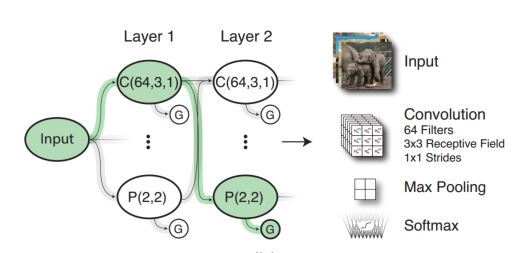
\includegraphics[width=0.85\textwidth]{adversarial_learning/images/qlearning.JPG}
    \label{fig:reinf_dnn}
    \caption{An example of reinforcement learning in deep neural networks: In green highlighted a path is shown, which the agent could select (based on MDPs) in the neural network. \cite{baker2016designing}.}
\end{figure}

\end{comment}

\subsection{Evolutionary Algorithms}
\label{evolutionaryalgorithms}
Evolutionary algorithms are based on the biological principle \textit{survival of the fittest}. Meaning, a population of individuals (e.g. solutions or scenarios) evolve through a sequence of evolutionary operators while trying to survive. After some generations, the surviving individuals represent a near-optimal solution.\\
Consequently, we want to find an individual $x \in \chi$ from an arbitrary set $\chi$ that minimizes a fitness function $f : \chi \rightarrow \mathbb{R}$. We assume that the best fitness has the lowest value. An evolutionary algorithm follows three steps \cite{michalewicz93}:
\begin{description}
   \begin{enumerate}
      \item Every $x \in \chi$ is evaluated to give some measure of its fitness score
      (Evaluation Step).
      \item A new population is formed by selecting the more fit individuals (Selection Step).
      \item Some members of the new population evolve through evolutionary operators to form new individuals. We denote $o:\mathfrak{P}(\chi)\rightarrow \mathfrak{P}(\chi)$ as the evolutionary step function so that $X_{i+1} = o(X_i)\forall i \ge 0$\\ (Alter Step).
   \end{enumerate}
\end{description}
Evolutionary operators usually follows mechanisms inspired by biological evolution. The biological operators, which are of relevance for this work are \cite{gabor19}:
\begin{description}
   \begin{itemize}
      \item \textit{recombination (rec)}: $\chi \times \chi \rightarrow \chi$ generates a new individual by combining parts of two given individuals.
      \item \textit{mutation (mut)}: $\chi \rightarrow \chi$ generates a new individual by making small changes in given individual.
      \item \textit{migration (mig)}: $\chi$ generates a random individual $mig \in \chi$
      \item \textit{selection (sel)}: $\mathfrak{P} (\chi) \times \mathbb{N} \rightarrow \mathfrak{P}(\chi)$ returns a new population\\
      $X' = sel(X,n)$ given a population $X \subseteq \chi$, so that $X' \le n$.
   \end{itemize}
\end{description}
With these steps the population should get fitter, i.e., $min_{x \in \chi_i} f(x) \ge min_{x \in \chi_i+k} f(x)$ for sufficiently large $k$. Ideally, the population converges to the best possible fitness at some point.

\subsection{Zero-sum Markov games}
\label{zerosumgames}

Zero-sum games simulate multi agent problems. The success of one agent is always the loss of the other. For example, in a two-player zero sum game, if one Agent gets a positive reward, the opponent gets an equal negative reward. This leads to the fact that the adversaries always pursue opposite goals. Payoff matrices in zero-sum games can be described as (M, -M). \inline{evtl beispiel matrizen zero-sum }
%https://neos-guide.org/content/game-theory-basics
In 2-player general-sum games (\textit{bimatrix games}) the solution depends on M\textsuperscript{1} as well as M\textsuperscript{2}, whereas in zero-sum games, the game can be simplified by using M or -M, the solution depends only on one of the two matrices. 2-player zero-sum games are therefore called \textit{matrix games}\cite{basics2hu1998multiagent}.

\[ 
\text{For all a\textsubscript{1}} \in A\textsubscript{1}, a \textsubscript{2} \in A\textsubscript{2}, \text{and s} \in S, R\textsubscript{1}(s, a\textsubscript{1}, a \textsubscript{2}) = - R\textsubscript{2}(s, a\textsubscript{1}, a \textsubscript{2})
\]
\\
where S is the set of states of the environment, A\textsubscript{n} is the collection of actions available to Agent n and $R\textsubscript{i}:S\times A\textsubscript{1}\times A\textsubscript{2} \Rightarrow \mathbb{R}$ is each agents reward function,  given the immediately expected reward obtained by agent \textit{i} for each selection of action sets that the group of agents could make in any state\cite{basics1littman1994markov}.\\
In a two-player zero sum game, there is actually only one reward function $R\textsubscript{1}$. Agent 1 tries to maximize it and Agent 2 tries to minimize it. Hence, zero-sum games are called adversarial or fully-competitive \cite{basics1littman1994markov}.\\
If both agents converge, we speak of a Nash Equilibrium.
In a Nash equilibrium, also called the \textit{saddle point}, each agent's choice is the best answer to the other agent's choice, resulting in no agent being able to obtain rewards through unilateral deviation\cite{nashgharesifard2013distributed, basics2hu1998multiagent}.


